“
–
’
 
\chapter{Interbranch quarrel in comparative perspective}
\label{ch:sopInPerspective}
\chaptermark{Comparative interbranch quarrel}

%abstract
%This chapter provides a birds-eye view on how I study the legislative process in systems of separation of power (sop).  Two decision-making principles coexist in sop: one requiring the powers to concur on new policy, another establishing exceptions to concurrent consent.  There is a tendency in the literature to overlook exceptions (unilateralism), biasing appraisals of sop systems.  The chapter also incorporates these principles into an abstract framework – the amplified game of sop – which represents the essential rules of policy-making.  The components of this game are isolated to get a sense of the substantive claims that can be produced with each.  The chapter also introduces a discussion on the motivation that guides politicians in choosing their actions.  Motivation will be the clue to begin constructing a unified model of the legislative process in systems of sop. 

There is a classic distinction in comparative politics between two forms of democratic government, the parliamentary and the presidential.  The primary attribute of parliamentarism is that the legislative and executive powers of government are fused; under presidentialism there is a separation of these powers \citep{lijphart.1984}. There has been much controversy over the pros and cons of fusion and separation of power.  

Debate has taken place mostly at the theoretical level, with claims remaining, for the most part, unaccompanied by convincing empirical evidence.  But even on the theoretical front the state of the discussion is inconclusive, due in great part to the difficulty of isolating the independent effect that broad governmental forms have on government performance from those of a myriad of smaller institutional details.  Asking whether fusion is better or worse than separation of power may be too broad a question.  

My research branches out of this intellectual tradition.  I shall not, however, engage in a discussion of pros and cons.  In this thesis I focus, instead, on \emph{how the legislative process operates in systems of separation of power in the Americas}.  Policy is, for the most part, written as a set of pieces of legislation.  The legislative process is consequently the primary arena where governmental actors make decisions affecting the citizenry.  

In this chapter I present an outline of my argument.  The chapter is divided into 9 short sections that are organized in the following fashion.  

\emph{Separation of Power}.  Section 1 situates decision-making in a presidential or “separation of power” system in the context of the establishment of checks and balances in government, highlighting the dilemmas this raises for constitutional designers.  A definition of separation of power will be found in this section.  Section 2 introduces two principles of decision-making that, I argue, characterize any system of separation of power.  The principles are concurrent consent and unilateralism.  Section 3 offers a quick critical assessment of the relevant literature; I argue that there is a tendency, especially acute in the comparative literature, to omit the institutions of unilateralism in their conception of the legislative process.  

The Legislative Process.  Next, I concentrate on sketching the conceptual tools for the study of the legislative process in a generic separation of power polity.  Section 4 introduces a general or macro framework – the amplified game of separation of power – knitting together the theoretical parts of my thesis (as well as theoretical extensions that I will develop in the near future).  I then break the big framework into three smaller, analytically tractable, subsidiary models, all of which branch off from the encompassing frame (they are sub-games).  Sections 5, 6, and 7 provide outlines of the subsidiary models: the setter sub-game; the conditional decree sub-game; and the vetoes in the shadow of decrees sub-game.  These sketches introduce the basic building blocks with which my succeeding arguments are constructed, and in each of these three sections I also discuss the interesting substantive claims that are made based on this sort of model, foreshadowing what I will do in subsequent chapters or future extensions of the work.  

Actors' motivation.  Section 8 begins by synthesizing the stylized structures in which politicians interact in my model.  I then introduce a discussion on motivation: what is it that moves politicians who play these stylized games of the legislative process?  This brief discussion will anticipate the contents of the final chapter of the thesis, an attempt to synthesize two literatures on the legislative process (one in Anglo-American politics, another in comparative politics) that do not communicate despite dealing with essentially the same issues.  

Section 9 concludes by summarizing my approach to the study of the legislative process into a research design, presenting the questions that guide the thesis, defining the dependent and main independent variables, establishing a null hypothesis, and offering a general description of the methodology.\footnote{As will be evident, I have written this introduction in such a way that it addresses the contents of a large research agenda.  Some parts of the argument are not developed in chapters to follow; I do indicate, nonetheless, which pieces of argument are developed in subsequent chapters and which are projects.}

\section{What is separation of power?}
\label{s:whatSOP}

In framing a government which is to be administered by men over men, 
the great difficulty lies in this: you must first enable the government to 
control the governed; and in the next place oblige it to control itself
—Madison (1788, Federalist 51). \nocite{madison.1788}

Political theorists for at least two and a half centuries have been seeking institutional devices to constrain the capacity of government to violate the rights of the citizenry.  Three eminent figures in this school of thought, \citet{locke.1690}, \citet{montesquieu.1748}, and \citet{madison.1788}, favored the separation of policy-making power as an effective way to curb the all-too-human inclination of rulers to exploit the ruled --- ``il faut que le pouvoir arr\^ete le pouvoir'' suggested the second (163), which the third translated almost literally as ``ambition must be made to counteract ambition'' (322).  Yet these thinkers were also the first to recognize what their detractors have subsequently been emphasizing \citep[eg.][]{bagehot.1867,wilson.1884,romero.1893}: if separation of power results in an increase in the representativeness of policy it also implies an inevitable loss in the government's decisiveness – perhaps, in the spirit of Madison, the central dilemma in democratic theory.  

Constitution-writers in the independent nations of the American continent, by following the example set forth by the U.S.\ at the end of the 18th century, seem to have valued increased representativeness more than they feared the possibility of governmental indecisiveness.  In drafting the institutions of government they chose to include checks and balances in some or all of four common modalities: (1) separation of legislative and executive powers; (2) separation of legislative power between two chambers representing different constituencies; (3) breaking policy into national and sub-national jurisdictions; and (4) separation of the enactment from the interpretation of law \citep[see][]{cox.mccubbins.2001,tsebelis.1995}. 

In this thesis I will be studying separation of power in the first modality only: the disjunction between the ability to write policy and the ability to turn it into law.  Constraining attention in this manner results in a narrow definition of separation of power throughout the thesis: \emph{by separation of power I will always mean separation of the legislative branch from the executive branch of government}.  In this sense, I am following the classic distinction I introduced at the opening of the chapter.  

By this definition, a separation of power system becomes synonymous with a presidential system.  I prefer the term ``separation of power'' (which I will often abbreviate as sop) because ``presidential'' is a term open to ambiguous meanings.\footnote{Thus for example, it is not uncommon for the literature to refer to a system with an abnormally strong or imperialist president as an excessively ``presidential'' one, or ``hyperpresidential''.  The literature, for example, refers to the centrality of Mexico's president as presidencialismo \citep{carpizo.1978,weldon.1997}. Yet by hyperpresidential, it could also be understood that the system in question boldly separates the authorities of the branches in a way that actually renders the president rather weak.  Sop avoids this confusion; I thank Matthew Shugart for pointing this out to me.}  In reviewing the literature, however, I retain the common term to make it easier to recognize original arguments.  

\section{Two decision-making principles in separation of power}
\sectionmark{Two decision-making principles}

The rules of separation of power are a mixture of two principles of decision-making that, in their pure form, are antithetical.  The principles in question are concurrent consent and unilateralism.  The principle of concurrent consent prescribes that new policy requires the approval of the two branches of government: any change in policy sought by the executive branch can be rejected or “vetoed” by the legislative branch; symmetrically, the executive can veto any proposal by the legislative.  The principle of unilateralism, on the other hand, allows one branch to overcome a rejection by the other: unilateral powers effectively entitle each branch to establish new policy by itself (under certain circumstances).  

In their pure form, it is easy to see that unilateralism and concurrent consent are mutually exclusive maxims.  Yet constitutional engineers over the last centuries have devised hybrid forms of these principles which can actually coexist.  This hybridization results in a mixture that may well be called concurrent consent with restricted unilateralism.  Below I argue that much of the debate on separation of power has failed to recognize the presence of elements of unilateralism in the structure of decision-making.  

Concurrent consent is incorporated into a sop constitution by empowering the legislative and the executive with an authority to veto new policy.  This gives rise to the executive veto and the congressional veto, faculties giving each branch the power to enforce the status quo ante before any new decision becomes law.  This mutual veto power is the feature of sop constitutions that is recognized by all scholarly literature, both of Anglo-American and comparative politics.  

Restricted unilateralism, on the other hand, is less often acknowledged as part of separation of power.  Restricted unilateralism is incorporated into a sop constitution in two main modalities, overrides and decrees.  

The override authority is the legislative branch’s means of setting aside an executive veto in order to clear the way for new policy.  An override mechanism becomes a restricted form of unilateralism by requiring the legislative assembly to reveal extraordinary strength before it is effective: if normal passage of policy requires a plurality of votes, overriding an executive veto typically requires a larger degree of consensus, some super-majority.  The larger the super-majority required, the more restricted becomes this form of unilateralism.  

The decree authority is the executive branch’s means of circumventing a congressional veto.  Executive decrees permit the president to set new policy without the need of a statute written by the legislative assembly \citep[9]{carey.shugart.1998}.  A decree is a restricted form of unilateralism because, after some time, the legislative branch may decide the fate of any executive decree.  The easier it is for the assembly to rescind or amend a decree, the more restricted becomes this form of unilateralism.  

\begin{table}
\begin{center}
\begin{tabular}{c|c|c}
\emph{Authority}        & \emph{Executive}             &  \emph{Legislative}              \\
\emph{by which$\ldots$} & \emph{branch}                &  \emph{branch}                   \\ \hline
$\ldots$ branch rejects & \textbf{executive veto}      & \textbf{legislative veto}        \\
a proposal              & Ch.\ 3 veto in US states     &  Ch.\ 9 reacting to executive    \\
by the other            & Ch.\ 5 stunts Chile/Mex.     &  decrees in Argentina            \\ \hline
$\ldots$ branch over-   & \textbf{unilateralism}       & \textbf{veto override}           \\
comes a rejection       & Ch.\ 6 urgency in Chile      &  Ch.\ 4 hopeless vetoes          \\
by the other            & Ch.\ 7 exec.\ coalition      &  Ch.\ 8 overrides in Brazil      \\
\end{tabular}
\caption{Veto power and unilateral provisions, side to side}\label{t:twoPrinciples}
\end{center}
\end{table}

Table \ref{t:twoPrinciples} summarizes how the two hybrid principles of decision-making are combined into the concept of separation of power that I use throughout this research.  Note that in this framework executive decrees are to legislative vetoes what veto overrides are to executive vetoes.  Both are concrete mechanisms by means of which concurrent consent and unilateralism are allocated, more or less symmetrically, to the branches of a separation-of-power government. 

Different separation of power systems can be thought of as mixtures of different proportions of concurrent consent and restricted unilateralism among the branches.  A sweeping literature documents the numerous dimensions over which the formal institutions of sop vary from one constitution to another \citep{shugart.carey.1992,mainwaring.shugart.1997,carey.shugart.1998}. So, for example, unilateralism is quite limited and lopsided towards the legislative branch in certain systems.  This is the case, for example, in the U.S., Mexico, and Costa Rica, where the executive has no formal decree authority to overcome a congressional veto, and where overrides of executive vetoes become effective only after two-thirds of each house of the assembly has voted favorably.  Other systems of sop have less limited and more symmetric unilateral provisions.  Examples of this are Brazil (since 1988) and Colombia (since 1991), where the executive is explicitly granted a decree-making authority and the legislative assembly is entitled to override vetoes more easily, by absolute majority only.  Still other systems tilt the balance of unilateral power towards the executive branch.  Such is the case in Argentina (since 1994), where the executive holds a decree power while the assembly’s override power requires a two-thirds vote \citep[150--5]{shugart.carey.1992}.

\section{Unilateralism overlooked: the pressure boiler and the safety valves}
\sectionmark{The pressure boiler and safety valves}

As I mentioned above, there is a remarkable tendency in the literature to ignore the presence of the restricted unilateralism principle in separation of power.  This tendency is milder and easier to account for in some works than in others.  The Anglo-American literature falls on the mild end: it does take one form of unilateralism into consideration but disregards the other.  Models of inter-branch relations in the U.S. typically feature the veto-override faculty of the assembly \citep{lee.1975,rohde.simon.1985}; they omit executive decree authority \citep[exceptions are][]{sala.1998,moe.howell.1999}.  Given that the U.S. constitution grants no formal decree authority to its executive, and that Anglo-American politics research focuses solely on the case of the U.S., it becomes easy to elucidate the omission of this form of unilateralism – it’s simply not needed to account for the case of the U.S.  

The tendency to neglect restricted unilateralism is starkest in the Perils of Presidentialism literature in the field of comparative politics.  This literature, largely derived from recent work by Juan Linz, has hypothesized the highly destabilizing potential of any presidential constitution.  Presidential systems, it is argued, by electing the branches of government separately and for fixed terms, promote discord between them; at the same time they fail to provide constitutional mechanisms to resolve such disputes \citep{linz.1990,linz.valenzuela.1994}.  Unilateralism, in both its forms, is discarded as part of the Linzian conception of SoP, and this has been inherited by the voluminous research that the framework inspired \citep{linz.valenzuela.1994}.  

The probable explanation behind this neglect of unilateral provisions is the search for parsimony.  Linz chose to explicitly ignore the smaller institutional details of SoP, as can be inferred from the following quote:

\begin{quote}
Without going into the \emph{complexities} of the relationship between the executive and the legislature in different presidential regimes, the relative dangers of predominance of one or the other, and the capacity to veto or stalemate decisions on legislation, there can be no doubt that presidential regimes are based on a dual democratic legitimacy and that no democratic principle can decide who represents the will of the people in principle \citep[][7, emphasis added]{linz.1994}.
\end{quote}

But, unlike the literature in the Anglo-American Politics field, the omission is puzzling in a comparative perspective.  In fact, the principal claim of those who first took issue with the Linzian argument is that we cannot really understand whether or not this double legitimacy is problematic, and to what extent, without paying attention to the “complexities” of separation of power \citep{shugart.carey.1992}.  The rebuttal to the Linzian literature has, in turn, motivated a voluminous research agenda \citep{mainwaring.shugart.1997}.  

A good analogy for the system of policy-making portrayed in the Linzian story seems to be a pressure boiler with no safety valve.\footnote{This evocative analogy was suggested to me by Gary Cox.}  Opposition between the executive and the legislative turns on the gas in the system, putting it under increasing pressure.  Pressure keeps accumulating as long as the branches maintain a disagreement about legislation.  In the absence of constitutional safety valves – i.e. mechanisms to shut off or depressurize the system in case the barometer approaches the red zone – the only way to bring pressure back to normal is by reaching an agreement between the branches – turning off the heat.  If recalcitrance between the branches prevails and no such agreement is reached, the whole system eventually blows up in a democratic meltdown.\footnote{Linz’s terms are, actually, pretty suggestive of this pressure boiler with missing safety valves: \begin{quote}who, on the basis of democratic principles, is better legitimated to speak in the name of the people: the president, or the congressional majority that opposes his policies?  [C]onflict is always latent and sometimes likely to erupt dramatically; there is no democratic principle to resolve it$\ldots$  It is therefore no accident that in some of those situations the military intervenes as “poder moderador” \citeyearpar[][7]{linz.1994}.\end{quote} On the contrary, when executive-legislative pressure becomes sizeable in a parliamentary system, a government crisis reunifies policy purpose between the executive and the legislature, ‘depressurizing’ the system.  This constitutional safety valve avoids the breakdown of democracy.}

The truth is, however, that the institutions of restricted unilateralism in fact equip sop systems with different sorts of devices to avoid explosions.  Legislative overrides, executive decrees, and other “complexities” that the Linzian story overlooked need to be brought back in: they constitute the very safety valves of the sop pressure boiler.\footnote{\citet{domingo.morgenstern.nd} list at least a dozen of other formal and informal “road-clearing devices”, such as congressional monopoly on constitutional amendment (as in Colombia); budgetary bills subject to no executive veto (as in Mexico); agenda-setting tools like the urgency provision in the hands of the executive (as in Chile); etc.}  In the following sections I introduce an alternative framework that takes the safety valves of presidentialism into consideration; this represents one important deviation from the Linzian structure.  

\section{The legislative process as a game of strategy}

How are decisions made under separation of power?  How do the institutions translating the principles of concurrent consent and unilateralism, described in previous sections, interplay?  In particular, how do the congressional and the executive veto powers, the veto-override provision, and executive decree authority determine policy outcomes?  What patterns can we expect from arrangements combining these institutions differently among the branches of government?  Answering these and related questions brings us straight into the realm of the legislative process.  The legislative process includes a wide range of actions leading to and including the enactment of statutes, passage of resolutions, issuing of decree-laws, nominations and confirmations, and so forth.  

I construe the legislative process as a game of strategy played by politicians.  I will call this stylized framework the amplified game of separation of power (or the amplified sop game for short).  Representing decision-making with the tools of game theory is standard procedure in analyses of U.S. politics \citep[eg.][]{shepsle.1979,ingberman.yao.1991,krehbiel.1996,cox.1999,mccarty.2000,cameron.2000}.  It is a much less common research strategy in comparative studies, though it is gaining popularity \citep[eg.][]{huber.1996a,cox.1997,diermeier.feddersen.1998,baron.ferejohn.1989,londregan.2000a}.  I choose the game theoretic approach to the structure and process of policy because it is a particularly useful one.  It forces the analyst to think systematically about who makes collective choices, what actions are available to “players” at different stages of the “game”, and which actions should be chosen in light of pre-defined goals.  Such representation, when used creatively, generates some non-evident and even counter-intuitive conclusions from a set of explicit primitives.  Moreover, deductive reasoning – inherited to game theory by its mathematical formalization – facilitates appraisal of the consequences of altering a model’s premises, while assuring that the argument remains logically sound.  

amplified sop is a game for three players.  It begins with a pre-established policy, the status quo (denoted by SQ), which players “P”, “L”, and “V” jointly decide whether or not to change under rules that I portray in Game Tree 1.1.  Player P represents the president; player L represents a unitary-actor legislature; and player V is the veto-override pivot (whose identity I clarify below).  

\begin{figure}
 \begin{center}
  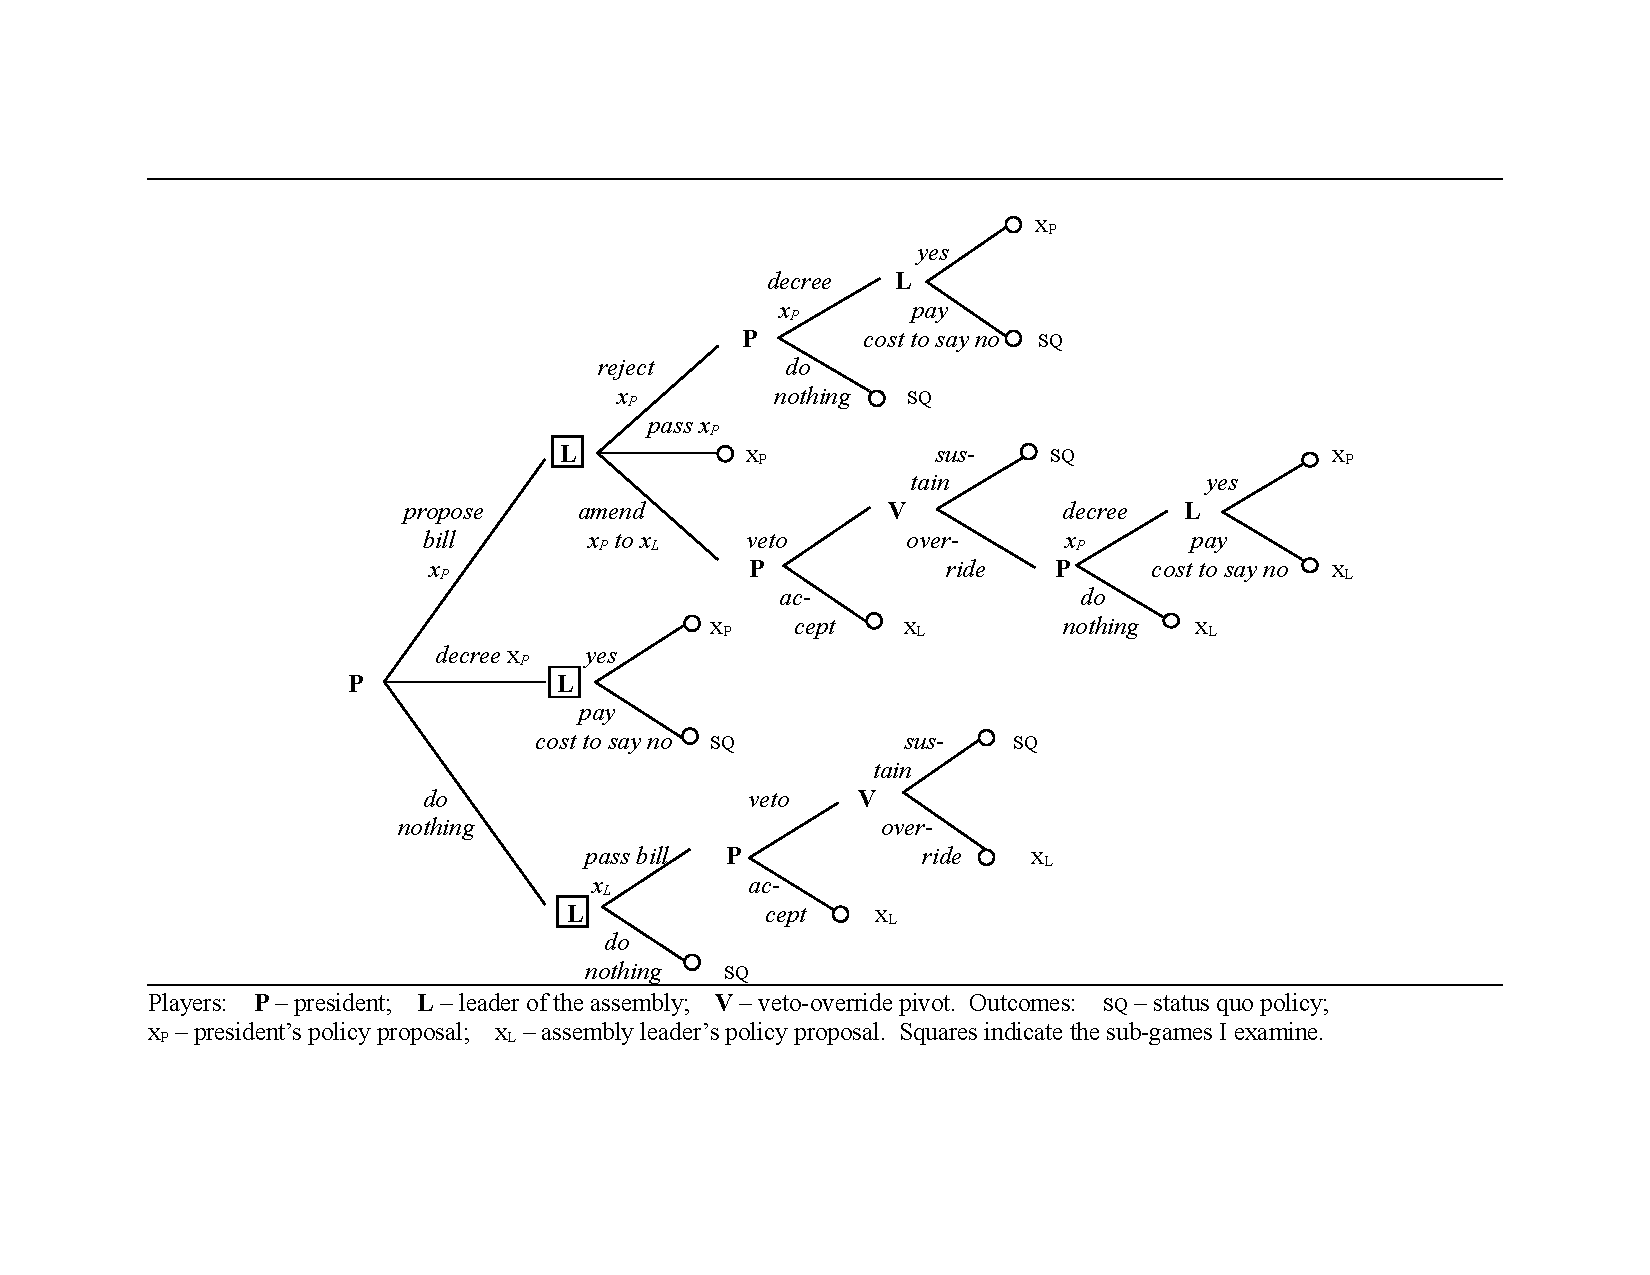
\includegraphics[width=\textwidth]{../veto/graphs/amplifiedGameOld.pdf}
 \caption{The big tree of separation of power: the amplified sop game}\label{f:amplifiedGame}
 \end{center}
\end{figure}

Player P starts the amplified sop game by choosing one of three available actions: P can propose a bill to the assembly; P can establish new policy by decree; or P can choose to do nothing.  The first choice represents an attempt by the president to make policy by statute (a change from the existing policy SQ to a new one denoted xP).\footnote{For clarification, no assumption is being made so far about the kind of bill proposed by player P; this will be the subject of subsequent chapters.  The subindex P in xP should only be interpreted as referring to the author of the policy proposal, in this case player P.  In the same fashion xL refers to a policy proposal by player L.}  The second choice represents an attempt by the president to establish the new policy xP unilaterally.  The third option represents a president who chooses to retain the status quo.  

Amplified sop ramifies into distinct sub-games depending on the action chosen by P in his or her first move.  I do not describe the sequence of action.  Instead I break exposition into some of the sub-games of amplified sop, devoting the following sections of the chapter to an outline of each (sub-games that I isolate from Game Tree 1.1 have a square in their starting node.)  Before doing so, however, a couple of comments are in order.  

Note first that the model involves an extremely simplified representation of the assembly.  I make collective choice in the amplified sop game analogous to choice by an individual, ignoring lessons against such a practice from the social choice literature \citep{plott.1967,mckelvey.1976,schofield.1983,riker.1980}. There are several ways of circumventing this problem.  One is to make feasible policies fall along a single dimension and then appeal to the median voter theorem to predict collective choice \citep{black.1958,tsebelis.money.1997}.  Another is to appeal to the presence exogenous restrictions that limit the social choice mechanism in a way that brings a stable and predictable equilibrium, such as transaction costs \citep{sloss.1973,lupia.mccubbins.1997} or the division of labor \citep{shepsle.1979}.  A plausible restriction to rely on is political parties as binding constraints that bring enough discipline among their members to render behavior by the collective body predictable \citep{cox.mccubbins.1994}. The elaboration of sub-games in chapters to follow involves unidimensionality; within this assumption, I leave it open for the reader to choose whether player L represents the leader of the party or coalition controlling a majority of seats \citep{cox.mccubbins.2005}, or the median member of a unicameral legislative assembly \citep{krehbiel.1998}.\footnote{If there is an advantage in having the majority in government then there exist good reasons to behave like a party.  There is evidence that majority status is valuable even in a system such as the U.S., where there is a consensus that parties are less meaningful than average.  Democrats lost between \$36,000 and \$60,000 per member in contributions from business PACs only upon losing grip of the House majority in 1994 \citep{cox.magar.1999,cox.magar.nd}.}

Second, let me tell what I will not be doing with this framework.  The principal object of a stylization of the legislative process such as the amplified sop game is to put the analyst in a position to generate interesting logical predictions.  This operation involves finding a game’s equilibria, something analogous to “solving” the game.  An equilibrium in the game is a set of mutual best-reply strategies (one for every player); stated differently, in equilibrium each player is responding optimally to what the others are doing.  Equilibria are obtained by logical deduction: they follow from a set of premises describing the game’s rules, a definition of what motivates every player in the game, and other elements of a more technical nature.  

So far I have provided some of the elements to obtain equilibrium strategies for the game.  I do not intend to solve the amplified sop game in this thesis.  The abundance of ramifications in Game Tree 1.1 yields countless possible combinations of moves, making their analysis a most burdensome task that I leave for the future; I have more modest goals at present.  Despite this, there are at least two good reasons why presenting the amplified sop game has been a useful exercise.  

One is that the richness of amplified sop is putting together several echelons of the legislative process that the literature has treated on a piecemeal basis, providing a useful synthesis.  The proactive and reactive legislative powers of presidents \citep{mainwaring.shugart.1997a}; executive decree authority \citep{carey.shugart.1998,remington.etal.1998}; and decision-theoretic approaches to presidential legislative choices \citep[eg.][]{amorim.1998} are all encapsulated in a single picture.  This encompassing frame follows almost literally the lines set forth in \citet{cox.morgenstern.1998} characterization of executive-legislative relations in Latin America as a distinctive sub-family of bilateral veto games (see especially pp.\ 3--4).  The tree also facilitates an extension into previous and posterior stages of the legislative process.  I do not carry this, but it seems easy to include the coalition-building process \citep{amorim.1998,deheza.1997} as taking place right before P’s first choice in amplified sop; the implementation of policy stage \citep{denhartog.2000,rosenblum.2000} can also be easily added as delegation following terminal nodes in Game Tree 1.1; popular initiative of legislation \citep{gerber.1996} is another development.  

Of more immediate value is the fact that I use the structure of amplified sop as an organizational tool for my thesis and some extensions that stem from it.  As pointed out, I break amplified sop into analytically-tractable sub-games, each of which serves as the basis to generate a set of interesting substantive claims.  Chapter 2 will actually consist of a full analysis and solution of the setter sub-game in which players are motivated by dual goals.  Chapter 4 contains the embryo of what will be a full analysis of the conditional decree sub-game; the chapter also presents evidence about the observed paths of play of amplified sop in Argentina.  The vetoes in the shadow of decrees sub-game will be a natural extension of this book.  I outline what the full development of each sub-game will look like in the three sections to follow.  

\section{The setter sub-game}

I start with a description of the sub-game of amplified sop located at the bottom of Game Tree 1.1.  This is the ramification that develops after a do nothing choice by player P the first move.  I refer to this sub-game as the setter sub-game, and portray its rules in Game Tree 1.2.  

\begin{figure}
  \begin{center}
    \tikzstyle{mid}=[circle,draw]
    \begin{tikzpicture}
      % \node[rectangle,draw] (n) at (0,0) {Nature};
      \node (n) at (0,0) {Nature: $\pi$}; \node[mid] at (2,0) (l)
      {\emph{l}}; \node[mid] at (4,1) (e) {\emph{e}}; \node[mid]
      at (6,0) (v) {\emph{v}}; \node at (4,-1) (le) {$x_0$}; \node
      at (6,2) (ee) {$x$}; \node at (8,1) (ve1) {$x_0$}; \node at
      (8,-1) (ve2) {$x$};
      % \node at (0,0.7) {\small{Strategies:}}; \node at (2,0.7)
      % {\footnotesize{---}}; \node at (4,0.7) {\footnotesize{$x^*$}};
      % \node at (6,0.7) {\footnotesize{$y^*(x)$}}; \node at (8,0.7)
      % {\footnotesize{$z^*(x)$}}; \node at (0,-1.7)
      % {\small{Outcomes:}};
      \path[->] (n) edge (l); \path[-] (l) edge node [above, sloped]
      {\footnotesize{pro-}} (e) (e) edge node [below, sloped]
      {\footnotesize{veto}} (v);
      % \path[] (n) edge node [below] {\footnotesize{$\pi$}} (l)
      \path[] (l) edge node [below, sloped] {\footnotesize{pose $x$}}
      (e); \path[-o] (l) edge node [below, sloped]
      {\footnotesize{not}} (le) (e) edge node [above, sloped]
      {\footnotesize{accept}} (ee) (v) edge node [above, sloped]
      {\footnotesize{sustain}} (ve1) edge node [above, sloped]
      {\footnotesize{over-}} (ve2) edge node [below, sloped]
      {\footnotesize{ride}} (ve2);
    \end{tikzpicture}
    \caption{The stunts game}\label{F:game}
  \end{center}
\end{figure}
